\documentclass{standalone}
\usepackage{tikz}
\usetikzlibrary{patterns, positioning}


\begin{document}
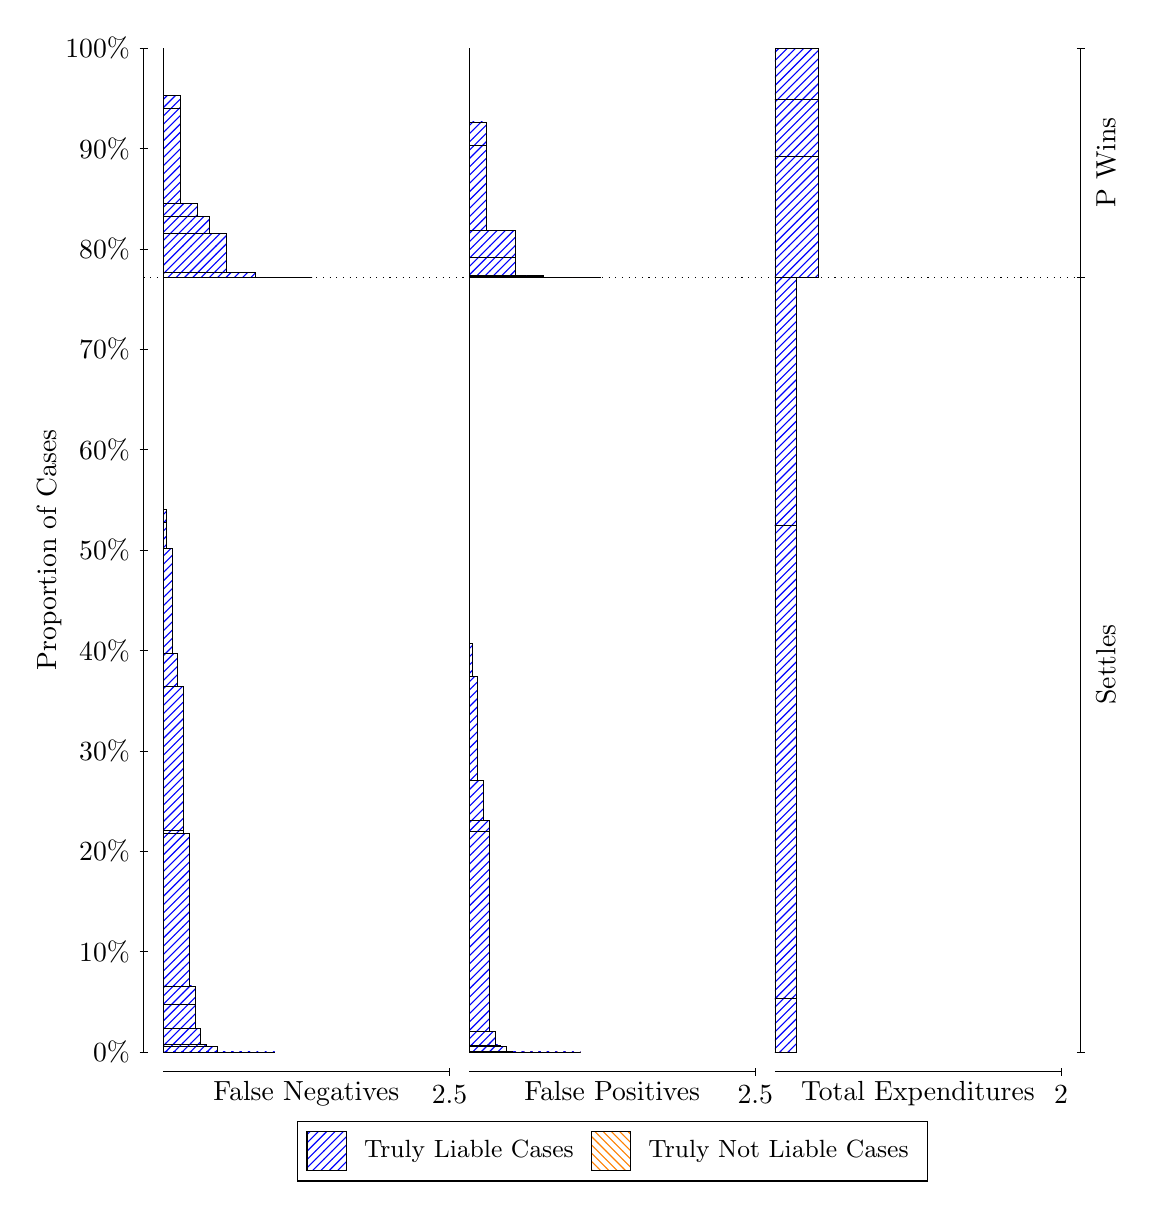
\begin{tikzpicture}
\draw[black, very thin] (1.5,1.75) -- (1.5,14.5);
\node[rotate=90, text=black, anchor=center] at (0.3, 8.125) {Proportion of Cases};
\draw[black, very thin] (1.45,1.75) -- (1.55,1.75);
\node[text=black, anchor=east] at (1.45, 1.75) {0\%};
\draw[black, very thin] (1.45,3.025) -- (1.55,3.025);
\node[text=black, anchor=east] at (1.45, 3.025) {10\%};
\draw[black, very thin] (1.45,4.3) -- (1.55,4.3);
\node[text=black, anchor=east] at (1.45, 4.3) {20\%};
\draw[black, very thin] (1.45,5.575) -- (1.55,5.575);
\node[text=black, anchor=east] at (1.45, 5.575) {30\%};
\draw[black, very thin] (1.45,6.85) -- (1.55,6.85);
\node[text=black, anchor=east] at (1.45, 6.85) {40\%};
\draw[black, very thin] (1.45,8.125) -- (1.55,8.125);
\node[text=black, anchor=east] at (1.45, 8.125) {50\%};
\draw[black, very thin] (1.45,9.4) -- (1.55,9.4);
\node[text=black, anchor=east] at (1.45, 9.4) {60\%};
\draw[black, very thin] (1.45,10.675) -- (1.55,10.675);
\node[text=black, anchor=east] at (1.45, 10.675) {70\%};
\draw[black, very thin] (1.45,11.95) -- (1.55,11.95);
\node[text=black, anchor=east] at (1.45, 11.95) {80\%};
\draw[black, very thin] (1.45,13.225) -- (1.55,13.225);
\node[text=black, anchor=east] at (1.45, 13.225) {90\%};
\draw[black, very thin] (1.45,14.5) -- (1.55,14.5);
\node[text=black, anchor=east] at (1.45, 14.5) {100\%};

\draw[black, very thin] (13.4,1.75) -- (13.4,14.5);
\draw[black, very thin] (13.35,1.75) -- (13.45,1.75);
\node[anchor=west] at (13.35, 1.75) {};
\draw[black, very thin] (13.35,11.59) -- (13.45,11.59);
\node[anchor=west] at (13.35, 11.59) {};
\draw[black, very thin] (13.35,14.5) -- (13.45,14.5);
\node[anchor=west] at (13.35, 14.5) {};

\draw[black, very thin, pattern color=blue, pattern=north east lines] (1.75,1.75) rectangle (3.167,1.75);
\draw[black, very thin, pattern color=blue, pattern=north east lines] (1.75,1.75) rectangle (2.8763,1.75);
\draw[black, very thin, pattern color=blue, pattern=north east lines] (1.75,1.75) rectangle (2.8037,1.75);
\draw[black, very thin, pattern color=blue, pattern=north east lines] (1.75,1.75) rectangle (2.731,1.75);
\draw[black, very thin, pattern color=blue, pattern=north east lines] (1.75,1.75) rectangle (2.5857,1.7504);
\draw[black, very thin, pattern color=blue, pattern=north east lines] (1.75,1.7504) rectangle (2.513,1.7521);
\draw[black, very thin, pattern color=blue, pattern=north east lines] (1.75,1.7521) rectangle (2.4403,1.8167);
\draw[black, very thin, pattern color=blue, pattern=north east lines] (1.75,1.8167) rectangle (2.3677,1.8179);
\draw[black, very thin, pattern color=blue, pattern=north east lines] (1.75,1.8179) rectangle (2.295,1.8479);
\draw[black, very thin, pattern color=blue, pattern=north east lines] (1.75,1.8479) rectangle (2.2223,2.049);
\draw[black, very thin, pattern color=blue, pattern=north east lines] (1.75,2.049) rectangle (2.1497,2.3571);
\draw[black, very thin, pattern color=blue, pattern=north east lines] (1.75,2.3571) rectangle (2.1497,2.5892);
\draw[black, very thin, pattern color=blue, pattern=north east lines] (1.75,2.5892) rectangle (2.077,4.5306);
\draw[black, very thin, pattern color=blue, pattern=north east lines] (1.75,4.5306) rectangle (2.0043,4.5624);
\draw[black, very thin, pattern color=blue, pattern=north east lines] (1.75,4.5624) rectangle (2.0043,6.3961);
\draw[black, very thin, pattern color=blue, pattern=north east lines] (1.75,6.3961) rectangle (1.9317,6.8169);
\draw[black, very thin, pattern color=blue, pattern=north east lines] (1.75,6.8169) rectangle (1.859,8.1428);
\draw[black, very thin, pattern color=blue, pattern=north east lines] (1.75,8.1428) rectangle (1.7863,8.4821);
\draw[black, very thin, pattern color=blue, pattern=north east lines] (1.75,8.4821) rectangle (1.7863,8.6469);
\draw[black, very thin, pattern color=orange, pattern=north west lines] (1.75,8.6469) rectangle (1.75,8.6469);
\draw[black, very thin, pattern color=blue, pattern=north east lines] (1.75,8.6469) rectangle (1.75,11.59);
\draw[black, very thin, pattern color=blue, pattern=north east lines] (1.75,11.59) rectangle (3.6393,11.59);
\draw[black, very thin, pattern color=blue, pattern=north east lines] (1.75,11.59) rectangle (3.276,11.591);
\draw[black, very thin, pattern color=blue, pattern=north east lines] (1.75,11.591) rectangle (3.058,11.591);
\draw[black, very thin, pattern color=blue, pattern=north east lines] (1.75,11.591) rectangle (2.9127,11.652);
\draw[black, very thin, pattern color=blue, pattern=north east lines] (1.75,11.652) rectangle (2.6947,11.652);
\draw[black, very thin, pattern color=blue, pattern=north east lines] (1.75,11.652) rectangle (2.5493,12.146);
\draw[black, very thin, pattern color=blue, pattern=north east lines] (1.75,12.146) rectangle (2.3313,12.365);
\draw[black, very thin, pattern color=blue, pattern=north east lines] (1.75,12.365) rectangle (2.186,12.527);
\draw[black, very thin, pattern color=blue, pattern=north east lines] (1.75,12.527) rectangle (1.968,13.73);
\draw[black, very thin, pattern color=blue, pattern=north east lines] (1.75,13.73) rectangle (1.968,13.903);
\draw[black, very thin, pattern color=blue, pattern=north east lines] (1.75,13.903) rectangle (1.8227,13.903);
\draw[black, very thin, pattern color=orange, pattern=north west lines] (1.75,13.903) rectangle (1.75,13.903);
\draw[black, very thin, pattern color=blue, pattern=north east lines] (1.75,13.903) rectangle (1.75,14.5);
\draw[black, very thin, pattern color=orange, pattern=north west lines] (5.6333,1.75) rectangle (7.0503,1.75);
\draw[black, very thin, pattern color=blue, pattern=north east lines] (5.6333,1.75) rectangle (7.0503,1.75);
\draw[black, very thin, pattern color=orange, pattern=north west lines] (5.6333,1.75) rectangle (6.905,1.75);
\draw[black, very thin, pattern color=blue, pattern=north east lines] (5.6333,1.75) rectangle (6.905,1.75);
\draw[black, very thin, pattern color=orange, pattern=north west lines] (5.6333,1.75) rectangle (6.7597,1.75);
\draw[black, very thin, pattern color=blue, pattern=north east lines] (5.6333,1.75) rectangle (6.7597,1.75);
\draw[black, very thin, pattern color=blue, pattern=north east lines] (5.6333,1.75) rectangle (6.687,1.75);
\draw[black, very thin, pattern color=orange, pattern=north west lines] (5.6333,1.75) rectangle (6.6143,1.75);
\draw[black, very thin, pattern color=blue, pattern=north east lines] (5.6333,1.75) rectangle (6.6143,1.75);
\draw[black, very thin, pattern color=blue, pattern=north east lines] (5.6333,1.75) rectangle (6.5417,1.75);
\draw[black, very thin, pattern color=orange, pattern=north west lines] (5.6333,1.75) rectangle (6.469,1.75);
\draw[black, very thin, pattern color=blue, pattern=north east lines] (5.6333,1.75) rectangle (6.469,1.75);
\draw[black, very thin, pattern color=blue, pattern=north east lines] (5.6333,1.75) rectangle (6.3963,1.75);
\draw[black, very thin, pattern color=orange, pattern=north west lines] (5.6333,1.75) rectangle (6.3237,1.75);
\draw[black, very thin, pattern color=blue, pattern=north east lines] (5.6333,1.75) rectangle (6.3237,1.7502);
\draw[black, very thin, pattern color=blue, pattern=north east lines] (5.6333,1.7502) rectangle (6.251,1.7505);
\draw[black, very thin, pattern color=orange, pattern=north west lines] (5.6333,1.7505) rectangle (6.1783,1.7505);
\draw[black, very thin, pattern color=blue, pattern=north east lines] (5.6333,1.7505) rectangle (6.1783,1.7549);
\draw[black, very thin, pattern color=blue, pattern=north east lines] (5.6333,1.7549) rectangle (6.1057,1.8185);
\draw[black, very thin, pattern color=blue, pattern=north east lines] (5.6333,1.8185) rectangle (6.033,1.8397);
\draw[black, very thin, pattern color=blue, pattern=north east lines] (5.6333,1.8397) rectangle (5.9603,2.0143);
\draw[black, very thin, pattern color=orange, pattern=north west lines] (5.6333,2.0143) rectangle (5.8877,2.0143);
\draw[black, very thin, pattern color=blue, pattern=north east lines] (5.6333,2.0143) rectangle (5.8877,4.5561);
\draw[black, very thin, pattern color=blue, pattern=north east lines] (5.6333,4.5561) rectangle (5.8877,4.693);
\draw[black, very thin, pattern color=blue, pattern=north east lines] (5.6333,4.693) rectangle (5.815,5.1971);
\draw[black, very thin, pattern color=blue, pattern=north east lines] (5.6333,5.1971) rectangle (5.7423,6.5231);
\draw[black, very thin, pattern color=blue, pattern=north east lines] (5.6333,6.5231) rectangle (5.6697,6.9439);
\draw[black, very thin, pattern color=blue, pattern=north east lines] (5.6333,6.9439) rectangle (5.6333,11.59);
\draw[black, very thin, pattern color=orange, pattern=north west lines] (5.6333,11.59) rectangle (7.3047,11.59);
\draw[black, very thin, pattern color=blue, pattern=north east lines] (5.6333,11.59) rectangle (7.3047,11.59);
\draw[black, very thin, pattern color=orange, pattern=north west lines] (5.6333,11.59) rectangle (6.9413,11.59);
\draw[black, very thin, pattern color=blue, pattern=north east lines] (5.6333,11.59) rectangle (6.9413,11.59);
\draw[black, very thin, pattern color=blue, pattern=north east lines] (5.6333,11.59) rectangle (6.9413,11.59);
\draw[black, very thin, pattern color=orange, pattern=north west lines] (5.6333,11.59) rectangle (6.578,11.59);
\draw[black, very thin, pattern color=blue, pattern=north east lines] (5.6333,11.59) rectangle (6.578,11.598);
\draw[black, very thin, pattern color=blue, pattern=north east lines] (5.6333,11.598) rectangle (6.578,11.613);
\draw[black, very thin, pattern color=orange, pattern=north west lines] (5.6333,11.613) rectangle (6.36,11.613);
\draw[black, very thin, pattern color=blue, pattern=north east lines] (5.6333,11.613) rectangle (6.36,11.613);
\draw[black, very thin, pattern color=orange, pattern=north west lines] (5.6333,11.613) rectangle (6.2147,11.613);
\draw[black, very thin, pattern color=blue, pattern=north east lines] (5.6333,11.613) rectangle (6.2147,11.846);
\draw[black, very thin, pattern color=blue, pattern=north east lines] (5.6333,11.846) rectangle (6.2147,12.187);
\draw[black, very thin, pattern color=orange, pattern=north west lines] (5.6333,12.187) rectangle (5.9967,12.187);
\draw[black, very thin, pattern color=blue, pattern=north east lines] (5.6333,12.187) rectangle (5.9967,12.187);
\draw[black, very thin, pattern color=blue, pattern=north east lines] (5.6333,12.187) rectangle (5.8513,13.263);
\draw[black, very thin, pattern color=blue, pattern=north east lines] (5.6333,13.263) rectangle (5.8513,13.563);
\draw[black, very thin, pattern color=orange, pattern=north west lines] (5.6333,13.563) rectangle (5.6333,13.563);
\draw[black, very thin, pattern color=blue, pattern=north east lines] (5.6333,13.563) rectangle (5.6333,14.5);
\draw[black, very thin, pattern color=orange, pattern=north west lines] (9.5167,1.75) rectangle (9.7892,1.75);
\draw[black, very thin, pattern color=blue, pattern=north east lines] (9.5167,1.75) rectangle (9.7892,2.4376);
\draw[black, very thin, pattern color=orange, pattern=north west lines] (9.5167,2.4376) rectangle (9.7892,2.4376);
\draw[black, very thin, pattern color=blue, pattern=north east lines] (9.5167,2.4376) rectangle (9.7892,8.4388);
\draw[black, very thin, pattern color=orange, pattern=north west lines] (9.5167,8.4388) rectangle (9.7892,8.4388);
\draw[black, very thin, pattern color=blue, pattern=north east lines] (9.5167,8.4388) rectangle (9.7892,11.59);
\draw[black, very thin, pattern color=orange, pattern=north west lines] (9.5167,11.59) rectangle (10.062,11.59);
\draw[black, very thin, pattern color=blue, pattern=north east lines] (9.5167,11.59) rectangle (10.062,13.126);
\draw[black, very thin, pattern color=orange, pattern=north west lines] (9.5167,13.126) rectangle (10.062,13.126);
\draw[black, very thin, pattern color=blue, pattern=north east lines] (9.5167,13.126) rectangle (10.062,13.844);
\draw[black, very thin, pattern color=orange, pattern=north west lines] (9.5167,13.844) rectangle (10.062,13.844);
\draw[black, very thin, pattern color=blue, pattern=north east lines] (9.5167,13.844) rectangle (10.062,14.5);
\draw[black, dotted] (1.5,11.59) -- (13.4,11.59);
\draw[black, very thin] (1.75,1.5) -- (5.3833,1.5);
\node[text=black, anchor=north] at (3.5667, 1.5) {False Negatives};
\draw[black, very thin] (5.3833,1.45) -- (5.3833,1.55);
\node[text=black, anchor=north] at (5.3833, 1.45) {2.5};

\draw[black, very thin] (5.6333,1.5) -- (9.2667,1.5);
\node[text=black, anchor=north] at (7.45, 1.5) {False Positives};
\draw[black, very thin] (9.2667,1.45) -- (9.2667,1.55);
\node[text=black, anchor=north] at (9.2667, 1.45) {2.5};

\draw[black, very thin] (9.5167,1.5) -- (13.15,1.5);
\node[text=black, anchor=north] at (11.333, 1.5) {Total Expenditures};
\draw[black, very thin] (13.15,1.45) -- (13.15,1.55);
\node[text=black, anchor=north] at (13.15, 1.45) {2};

\node[text=black, centered, rotate=90] at (13.72, 6.67) {Settles};
\node[text=black, centered, rotate=90] at (13.72, 13.045) {P Wins};

\draw (7.449999999999999,1.5) node[draw=none] (baseCoordinate) {};
\begin{scope}[align=center]
        \matrix[scale=0.5, draw=black, below=0.5cm of baseCoordinate, nodes={draw}, column sep=0.1cm]{
            \node[rectangle, draw, minimum width=0.5cm, minimum height=0.5cm, pattern color=blue, pattern=north east lines] {}; &
            \node[draw=none, font=\small, text=black] (B) {Truly Liable Cases}; &
            \node[rectangle, draw, minimum width=0.5cm, minimum height=0.5cm, pattern color=orange, pattern=north west lines] {}; &
            \node[draw=none, font=\small, text=black] (B) {Truly Not Liable Cases}; \\
            };
\end{scope}

\end{tikzpicture}
\end{document}